\documentclass[a4paper,10pt]{article}

\usepackage{geometry}
\geometry{a4paper,margin=1.4cm,top=1.2cm,bottom=1.2cm}

\usepackage{amsmath,amssymb}
\usepackage{xcolor}
\usepackage{array}
\usepackage{colortbl}
\usepackage{enumitem}
\usepackage{graphicx}
\usepackage{float}
\graphicspath{{../figs/synthesis/}}

\usepackage[extrafootnotefeatures]{xepersian}

\settextfont[
Scale=1.0,
Extension=.ttf,
Path=/Users/macbook/develope/thesis/thesis_latex/first_edition/styles/fonts/,
BoldFont=XB NiloofarBd,
ItalicFont=XB NiloofarIt,
BoldItalicFont=XB NiloofarBdIt
]{XB Niloofar}

\setdigitfont[
Scale=1.0,
Extension=.ttf,
Path=/Users/macbook/develope/thesis/thesis_latex/first_edition/styles/fonts/,
BoldFont=XB NiloofarBd
]{XB Niloofar}

\pagestyle{empty}
\setlength{\parindent}{0pt}
\setlength{\parskip}{2pt}

\definecolor{cok}{HTML}{2E6B4F}
\definecolor{cwarn}{HTML}{B5761A}
\definecolor{cred}{HTML}{B02020}
\definecolor{cgy}{HTML}{6A6A6A}
\definecolor{inkk}{HTML}{1A1A1A}
\definecolor{chd}{HTML}{2C5F8A}

\newcommand{\bul}{\ensuremath{\bullet}~}
\newcommand{\done}{{\color{cok}\bfseries نوشته‌شده}}
\newcommand{\wip}{{\color{cwarn}\bfseries ناقص}}
\newcommand{\todo}{{\color{cred}\bfseries نوشته‌نشده}}

\newcommand{\hd}[1]{%
  \vspace{4pt}%
  {\color{chd}\rule{\linewidth}{1pt}}\\[1pt]
  {\large\bfseries\color{chd} #1}\\[1pt]
  {\color{chd}\rule{\linewidth}{0.4pt}}\\[2pt]}

\newcommand{\sub}[1]{\vspace{2pt}{\bfseries\color{inkk} #1}\\[1pt]}

\renewcommand{\arraystretch}{1.15}

\begin{document}

\begin{center}
{\LARGE\bfseries گزارش وضعیت پایان‌نامه}\\[3pt]
{\small\color{cgy} کاهش شکاف دقت بخش‌بندی چندعضوی میان فاز بدون‌کنتراست و کنتراست‌دار در سی‌تی شکمی \raisebox{1pt}{---} ۱۵ شهریور ۱۴۰۵}
\end{center}
\vspace{-4pt}

% =====================================================================
\hd{۱. وضعیت نگارش}

دو فصل اول  نوشته ‌شده و نیاز به بازنگری پایانی متن اصلی دارد.

فصل سوم و چهارم هنوز کامل نشده‌اندو فقط جزئیات نحوه‌ی گزارش نتایج مانده‌است.

فصل پنجم (نتیجه‌گیری) هنوز نوشته نشده است.



% =====================================================================
\hd{۲. وضعیت نتایج}

\sub{زیرمسئله ۱ \raisebox{1pt}{---} مرور نظام‌مند مجموعه‌داده‌ها}
۴۵ مجموعه‌داده و ۴۷٬۰۴۹ بررسی فهرست‌شده که تنها ۲۳٬۷۴۶ مورد (۵۰٫۵ درصد) اصیل‌اند؛ ۷۵٫۳ درصد مجموعه‌داده‌ها از آمریکای شمالی و اروپا؛ ارزیابی ریسک سوگیری روی ۲۲ مجموعه‌داده کامل شده است (سوگیری نژادی ۱۶ از ۲۲، سوگیری انتخاب ۱۵ از ۲۲).


\sub{زیرمسئله ۲ \raisebox{1pt}{---} تشخیص فاز کنتراست‌دار}
انتخاب مدل طبقه‌بند \lr{XGBoost} روی بردار ۱۶ بعدی میانه‌ی \lr{HU} در سطح اندام، با اعتبارسنجی متقاطع پنج‌لایه‌ای روی ۳۳۴ نمونه: دقت و میانگین کلان \lr{F1} در بازه‌ی ۰٫۹۱ تا ۱٫۰۰ بعنوان یک معیار ارزیابی در تسک سنتز فاز کنتراست دار
 وهمینطور معرفی مدلی بدون نیاز به خروجی‌های مدل سگمنتیشن برای تشخیص فاز.



\sub{زیرمسئله ۳ \raisebox{1pt}{---} ثبت تصویر بین‌فازی}
ارزیابی روی ۲۶ بررسی متناظر (۵۵ جفت فاز، ۵۸۱ سه‌تایی). روش پیشنهادی دایس ۰٫۸۱۶ و مرکز جرم ۲٫۱۲ میلی‌متر با صفر درصد تاخوردگی می‌گیرد. \lr{DEEDS} با ۰٫۸۸۶ به‌طور قاطع دقیق‌تر است ($p = 1.1\times10^{-86}$) اما ۲٫۶۵ درصد تاخوردگی دارد؛ در برابر \lr{uniGradICON} نتیجه مساوی است ($p = 0.45$). نتیجه‌ی مثبت کلیدی: پیش‌پردازش این پایان‌نامه به‌عنوان جلوبَند، دقت \lr{DEEDS} و \lr{uniGradICON} را نیز بالا می‌برد.

\sub{زیرمسئله ۴ \raisebox{1pt}{---} سنتز فاز کنتراست‌دار}
ارزیابی پایین‌دستی زوجی روی ۲۰ مورد آزمون در برابر هشت بازو. \lr{PLC-Net} روی ورید باب \lr{+0.1663} دایس نسبت به کف بدون‌کنتراست می‌گیرد و در هر ۲۰ مورد از ۲۰ مورد بهتر است؛ اثر خالص پس از کسر هزینه‌ی اسکلتی \lr{+0.052}. مقایسه با پنج روش منتشرشده انجام شده (بهتر از \lr{pix2pixHD}، \lr{CycleGAN}، \lr{CyTran} و \lr{DDPM}؛ هم‌ارز با \lr{ResViT} در حاشیه‌ی ۰٫۰۲ دایس). آزمون کنترل فاز، کالیبراسیون سطح، اعتبارسنجی معیارها، مطالعه‌ی برداشتی، شاهد کیفیت داده و تحلیل شکست کیسه‌ی صفرا همگی گزارش شده‌اند.

\newpage

% =====================================================================
\hd{۳. مطالبی که قرار است گفته شود}

\sub{ادعاهایی که شواهد از آن‌ها پشتیبانی می‌کند}
\begin{itemize}[leftmargin=1.1cm,itemsep=1pt,topsep=1pt]
\item \textbf{شکاف دقت واقعی است اما متمرکز است و نه یکنواخت.} اثر روی ورید باب بزرگ (\lr{+0.166}) و روی پارانشیم کبد و طحال و کلیه عملاً صفر است. این همان چیزی است که فیزیک مسئله پیش‌بینی می‌کند.
\item \textbf{محدودسازی دامنه‌ی معیار تراز به نقاب اندام کار می‌کند}، و دقیقاً در همان گروه‌های اندامی که فرضیه پیش‌بینی کرده بود و نه در گروه شاهد.
\item \textbf{دو گذر صلب نخست اثرهای مکمل دارند}: گذر صفر روی بافت پارانشیمی ($p = 7\times10^{-17}$) و گذر یک روی ساختار اسکلتی ($p = 3.6\times10^{-10}$). هیچ‌یک جایگزین دیگری نیست.
\item \textbf{دروازه‌های پذیرش، یک گذر مضر را به یک گذر بی‌اثر تبدیل کردند}؛ گذر دو در ۹۹٫۴ درصد ثبت‌ها رد شد و بدون دروازه خطا را شش برابر می‌کرد.
\item \textbf{پیش‌پردازش این پایان‌نامه ترکیب‌پذیر است}: دقت روش‌های موجود را نیز به‌طور معنادار بالا می‌برد. این ادعایی مستقل از رقابت با آن‌هاست.
\item \textbf{سطح تقویت از تصویر بدون‌کنتراست قابل استنتاج نیست} ($R^2 = -0.105$)؛ یک محدودیت ذاتی است و تنها راه، دریافت سطح به‌عنوان ورودی. این پشتوانه‌ی نظری شرط سطح است.
\item \textbf{فروپاشی شرط‌گذاری اندازه‌گیری شده و سازوکارش شناسایی شده است}: بردار شرط سطح خودش ۹۴٫۲ درصد اطلاعات فاز را حمل می‌کند. نسخه‌ی دوبعدی فاز را نگه داشت و سطح را میرا کرد؛ نسخه‌ی ۲٫۵ بعدی برعکس.
\item \textbf{یک یافته‌ی روش‌شناختی مستقل:} \lr{featHU} سودمندی پایین‌دستی را پیش‌بینی می‌کند و \lr{FID} نمی‌کند. معیارهای متعارف در این مسئله گمراه‌کننده‌اند.
\end{itemize}

% =====================================================================

\newpage

% =====================================================================
\hd{۴. جدول‌های نتیجه \raisebox{1pt}{---} زیرمسئله ۴ (سنتز)}

\sub{۴٫۱ اثر سنتز بر بخش‌بندی پایین‌دستی}
تفاوت زوجی میانگین دایس نسبت به بازوی \lr{ncct} روی ۲۰ مورد آزمون. مرجع، خروجی \lr{TotalSegmentator} روی تصویر \emph{واقعی} کنتراست‌دار است. ستون «اسکلتی» شاهد منفی است: کنتراست بر استخوان اثری ندارد، پس هر افتی در آن ستون هزینه‌ی \emph{خودِ تولید} است. ستون «خالص» همان سود عروقی منهای این هزینه است.

\vspace{2pt}
\begin{center}
\footnotesize
\begin{tabular}{|l|c|c|c|c|c|}
\hline
\rowcolor{black!6}
\textbf{بازو} & \textbf{ورید باب} & \textbf{عروقی} & \textbf{اسکلتی (هزینه)} & \textbf{خالص} & \textbf{موارد بهتر} \\
\hline
\lr{PLC-Net} (پیشنهادی) & \textbf{\lr{+0.1663}} & \textbf{\lr{+0.0381}} & \lr{-0.0142} & \textbf{\lr{+0.0523}} & \lr{20/20} \\
\hline
\lr{ResViT} & \lr{+0.1749} & \lr{+0.0345} & \lr{-0.0188} & \lr{+0.0533} & \lr{20/20} \\
\hline
\lr{l1\_organ\_groupnorm} (ابلیشن) & \lr{+0.1643} & \lr{+0.0438} & \lr{-0.0097} & \lr{+0.0535} & \lr{19/20} \\
\hline
\lr{PLC-Net} ۲٫۵ بعدی & \lr{+0.1312} & \lr{+0.0270} & \lr{-0.0183} & \lr{+0.0453} & \lr{19/20} \\
\hline
\lr{pix2pixHD} & \lr{+0.0997} & \lr{+0.0231} & \lr{-0.0084} & \lr{+0.0315} & \lr{19/20} \\
\hline
\lr{CycleGAN} & \lr{+0.0733} & \lr{+0.0089} & \lr{-0.0121} & \lr{+0.0210} & \lr{15/20} \\
\hline
\lr{CyTran} & \lr{-0.0087} & \lr{-0.0171} & \lr{-0.0137} & {\color{cred}\lr{-0.0034}} & \lr{7/20} \\
\hline
\lr{DDPM} & \lr{-0.0847} & \lr{-0.0358} & \lr{-0.0172} & {\color{cred}\lr{-0.0185}} & \lr{3/20} \\
\hline
\end{tabular}
\end{center}

{\small\color{cgy} هزینه‌ی تولید با سود عروقی هم‌بسته نیست (اسپیرمن $\rho = +0.32$، $p = 0.22$) و دامنه‌اش تنها ۲٫۳ برابر است؛ پس تفریق آن مجاز است و بازوهای پرآسیب را نظام‌مند جریمه نمی‌کند.}

\vspace{4pt}
\sub{۴٫۲ معیارهای وفاداری تصویری \raisebox{1pt}{---} همان هشت بازو، همان ترتیب}
همه روی دامنه‌ی مشترک \lr{HU[-200,400]}. \lr{oMAE} خطای مطلق درون نواحی اندام، \lr{featHU} خطای میانه‌ی عدد هانسفیلد (واحد \lr{HU})، و «فاز» دقت طبقه‌بند مستقل زیرمسئله ۲ روی خروجی سنتزی است.

\vspace{2pt}
\begin{center}
\footnotesize
\begin{tabular}{|l|c|c|c|c|c|c|c|}
\hline
\rowcolor{black!6}
\textbf{بازو} & \lr{PSNR}$\uparrow$ & \lr{SSIM}$\uparrow$ & \lr{oMAE}$\downarrow$ & \lr{featHU}$\downarrow$ & \lr{LPIPS}$\downarrow$ & \lr{FID}$\downarrow$ & \textbf{فاز}$\uparrow$ \\
\hline
\lr{PLC-Net} (پیشنهادی) & \lr{29.64} & \lr{0.937} & \lr{0.0332} & \lr{14.6} & \lr{0.040} & \lr{9.6} & \textbf{\lr{1.00}} \\
\hline
\lr{ResViT} & \lr{29.18} & \lr{0.929} & \lr{0.0349} & \lr{15.2} & \lr{0.057} & \lr{12.9} & \lr{1.00} \\
\hline
\lr{l1\_organ\_groupnorm} (ابلیشن) & \textbf{\lr{30.66}} & \textbf{\lr{0.949}} & \textbf{\lr{0.0286}} & \textbf{\lr{12.9}} & \lr{0.047} & \lr{28.3} & \lr{1.00} \\
\hline
\lr{PLC-Net} ۲٫۵ بعدی & \lr{28.95} & \lr{0.933} & \lr{0.0381} & \lr{22.0} & \lr{0.049} & \lr{16.7} & {\color{cred}\lr{0.75}} \\
\hline
\lr{pix2pixHD} & \lr{30.01} & \lr{0.941} & \lr{0.0319} & \lr{17.1} & \textbf{\lr{0.038}} & \textbf{\lr{7.6}} & \lr{0.95} \\
\hline
\lr{CycleGAN} & \lr{29.88} & \lr{0.938} & \lr{0.0335} & \lr{18.7} & \lr{0.052} & \lr{11.1} & \lr{1.00} \\
\hline
\lr{CyTran} & \lr{28.87} & \lr{0.930} & \lr{0.0451} & {\color{cred}\lr{38.1}} & \lr{0.052} & \lr{10.4} & {\color{cred}\lr{0.35}} \\
\hline
\lr{DDPM} & \lr{28.74} & \lr{0.934} & \lr{0.0392} & \lr{24.8} & \lr{0.055} & \lr{18.3} & \lr{1.00} \\
\hline
\end{tabular}
\end{center}

{\small\color{cgy} این جدول را باید کنار جدول ۴٫۱ خواند. \lr{pix2pixHD} بهترین \lr{FID} و \lr{LPIPS} کل مطالعه را دارد و در اثر پایین‌دستی پایین‌تر از سه بازو با \lr{FID} بدتر است؛ و ابلیشن تک‌فاز، بدترین \lr{FID} این گروه را دارد و بالاترین اثر پایین‌دستی را. کل دامنه‌ی \lr{PSNR} میان هشت بازو ۱٫۹ دسی‌بل است، در حالی که اثر پایین‌دستی از \lr{-0.019} تا \lr{+0.054} پخش است.}

\vspace{4pt}
\sub{۴٫۳ اعتبار معیارها \raisebox{1pt}{---} کدام معیار سودمندی را پیش‌بینی می‌کند؟}
هم‌بستگی اسپیرمن هر معیار وفاداری با اثر خالص پایین‌دستی، روی ۱۶ بازوی وریدی. معیارها چنان جهت‌دهی شده‌اند که بزرگ‌تر همیشه بهتر باشد. ستون دوم آزمون مقاومت است: با کنارگذاشتن سه بازوی فروپاشیده (\lr{DDPM}، \lr{CyTran}، ۲٫۵ بعدی آخرین وزن).

\vspace{2pt}
\begin{center}
\footnotesize
\begin{tabular}{|l|c|c|l|}
\hline
\rowcolor{black!6}
\textbf{معیار} & \textbf{$\rho$ (همه، \lr{n=16})} & \textbf{$\rho$ (بدون فروپاشیده‌ها، \lr{n=13})} & \textbf{حکم} \\
\hline
\lr{featHU} & \textbf{\lr{+0.81}} ($p=0.0001$) & \textbf{\lr{+0.68}} ($p=0.010$) & {\color{cok}\bfseries مقاوم؛ تنها معیار پایدار} \\
\hline
\lr{MAE} اندامی & \lr{+0.64} & \lr{+0.36} ($p=0.23$) & فقط با حضور شکست‌ها \\
\hline
\lr{PSNR} & \lr{+0.58} & --- & فقط با حضور شکست‌ها \\
\hline
\lr{SSIM} اندامی & \lr{+0.56} & --- & فقط با حضور شکست‌ها \\
\hline
\lr{LPIPS} & \lr{+0.44} & \lr{+0.18} ($p=0.57$) & فقط با حضور شکست‌ها \\
\hline
\lr{FID (Rad)} & \lr{+0.20} & --- & بدون قدرت پیش‌بینی \\
\hline
\lr{RAPS} & \lr{+0.04} & --- & بدون قدرت پیش‌بینی \\
\hline
\lr{FID} & {\color{cred}\lr{-0.19}} ($p=0.47$) & --- & {\color{cred}\bfseries علامت وارونه} \\
\hline
\end{tabular}
\end{center}

{\small\color{cgy} ادعای دقیق: \lr{featHU} به‌طور مقاوم سودمندی پایین‌دستی را پیش‌بینی می‌کند؛ سایر معیارهای وفاداری تنها زمانی چنین به نظر می‌رسند که مدل‌های فاجعه‌بار در نمونه حاضر باشند؛ و \lr{FID} هرگز چنین نمی‌کند.}

\newpage

% =====================================================================
\hd{۵. شکل‌های شاهد}

{\small\color{cgy} قرارداد مشترک همه‌ی شکل‌ها: مرجع، خروجی \lr{TotalSegmentator} روی تصویر \emph{واقعی} کنتراست‌دار است (نه حاشیه‌نویسی انسانی) و هر عدد یک مقایسه‌ی \emph{زوجی} با بازوی \lr{ncct} روی همان ۲۰ مورد است. ستاره‌ها: \lr{***} یعنی $p<0.001$.}

\vspace{4pt}
\sub{۵٫۱ اثر سنتز کجا ظاهر می‌شود}
اندام‌ها بر حسب دایسشان روی تصویر بدون‌کنتراست مرتب شده‌اند، پس آناتومی‌ای که کنتراست بیشترین نقش را در آن دارد پایین نمودار است. نشانگر توپر یعنی معنادار، تُهی یعنی غیرمعنادار؛ لوزی‌ها مدل‌های پیشنهادی‌اند. نوار خاکستری، آناتومی اسکلتی و عضلانی یعنی شاهد منفی است.

\begin{figure}[H]
\centering
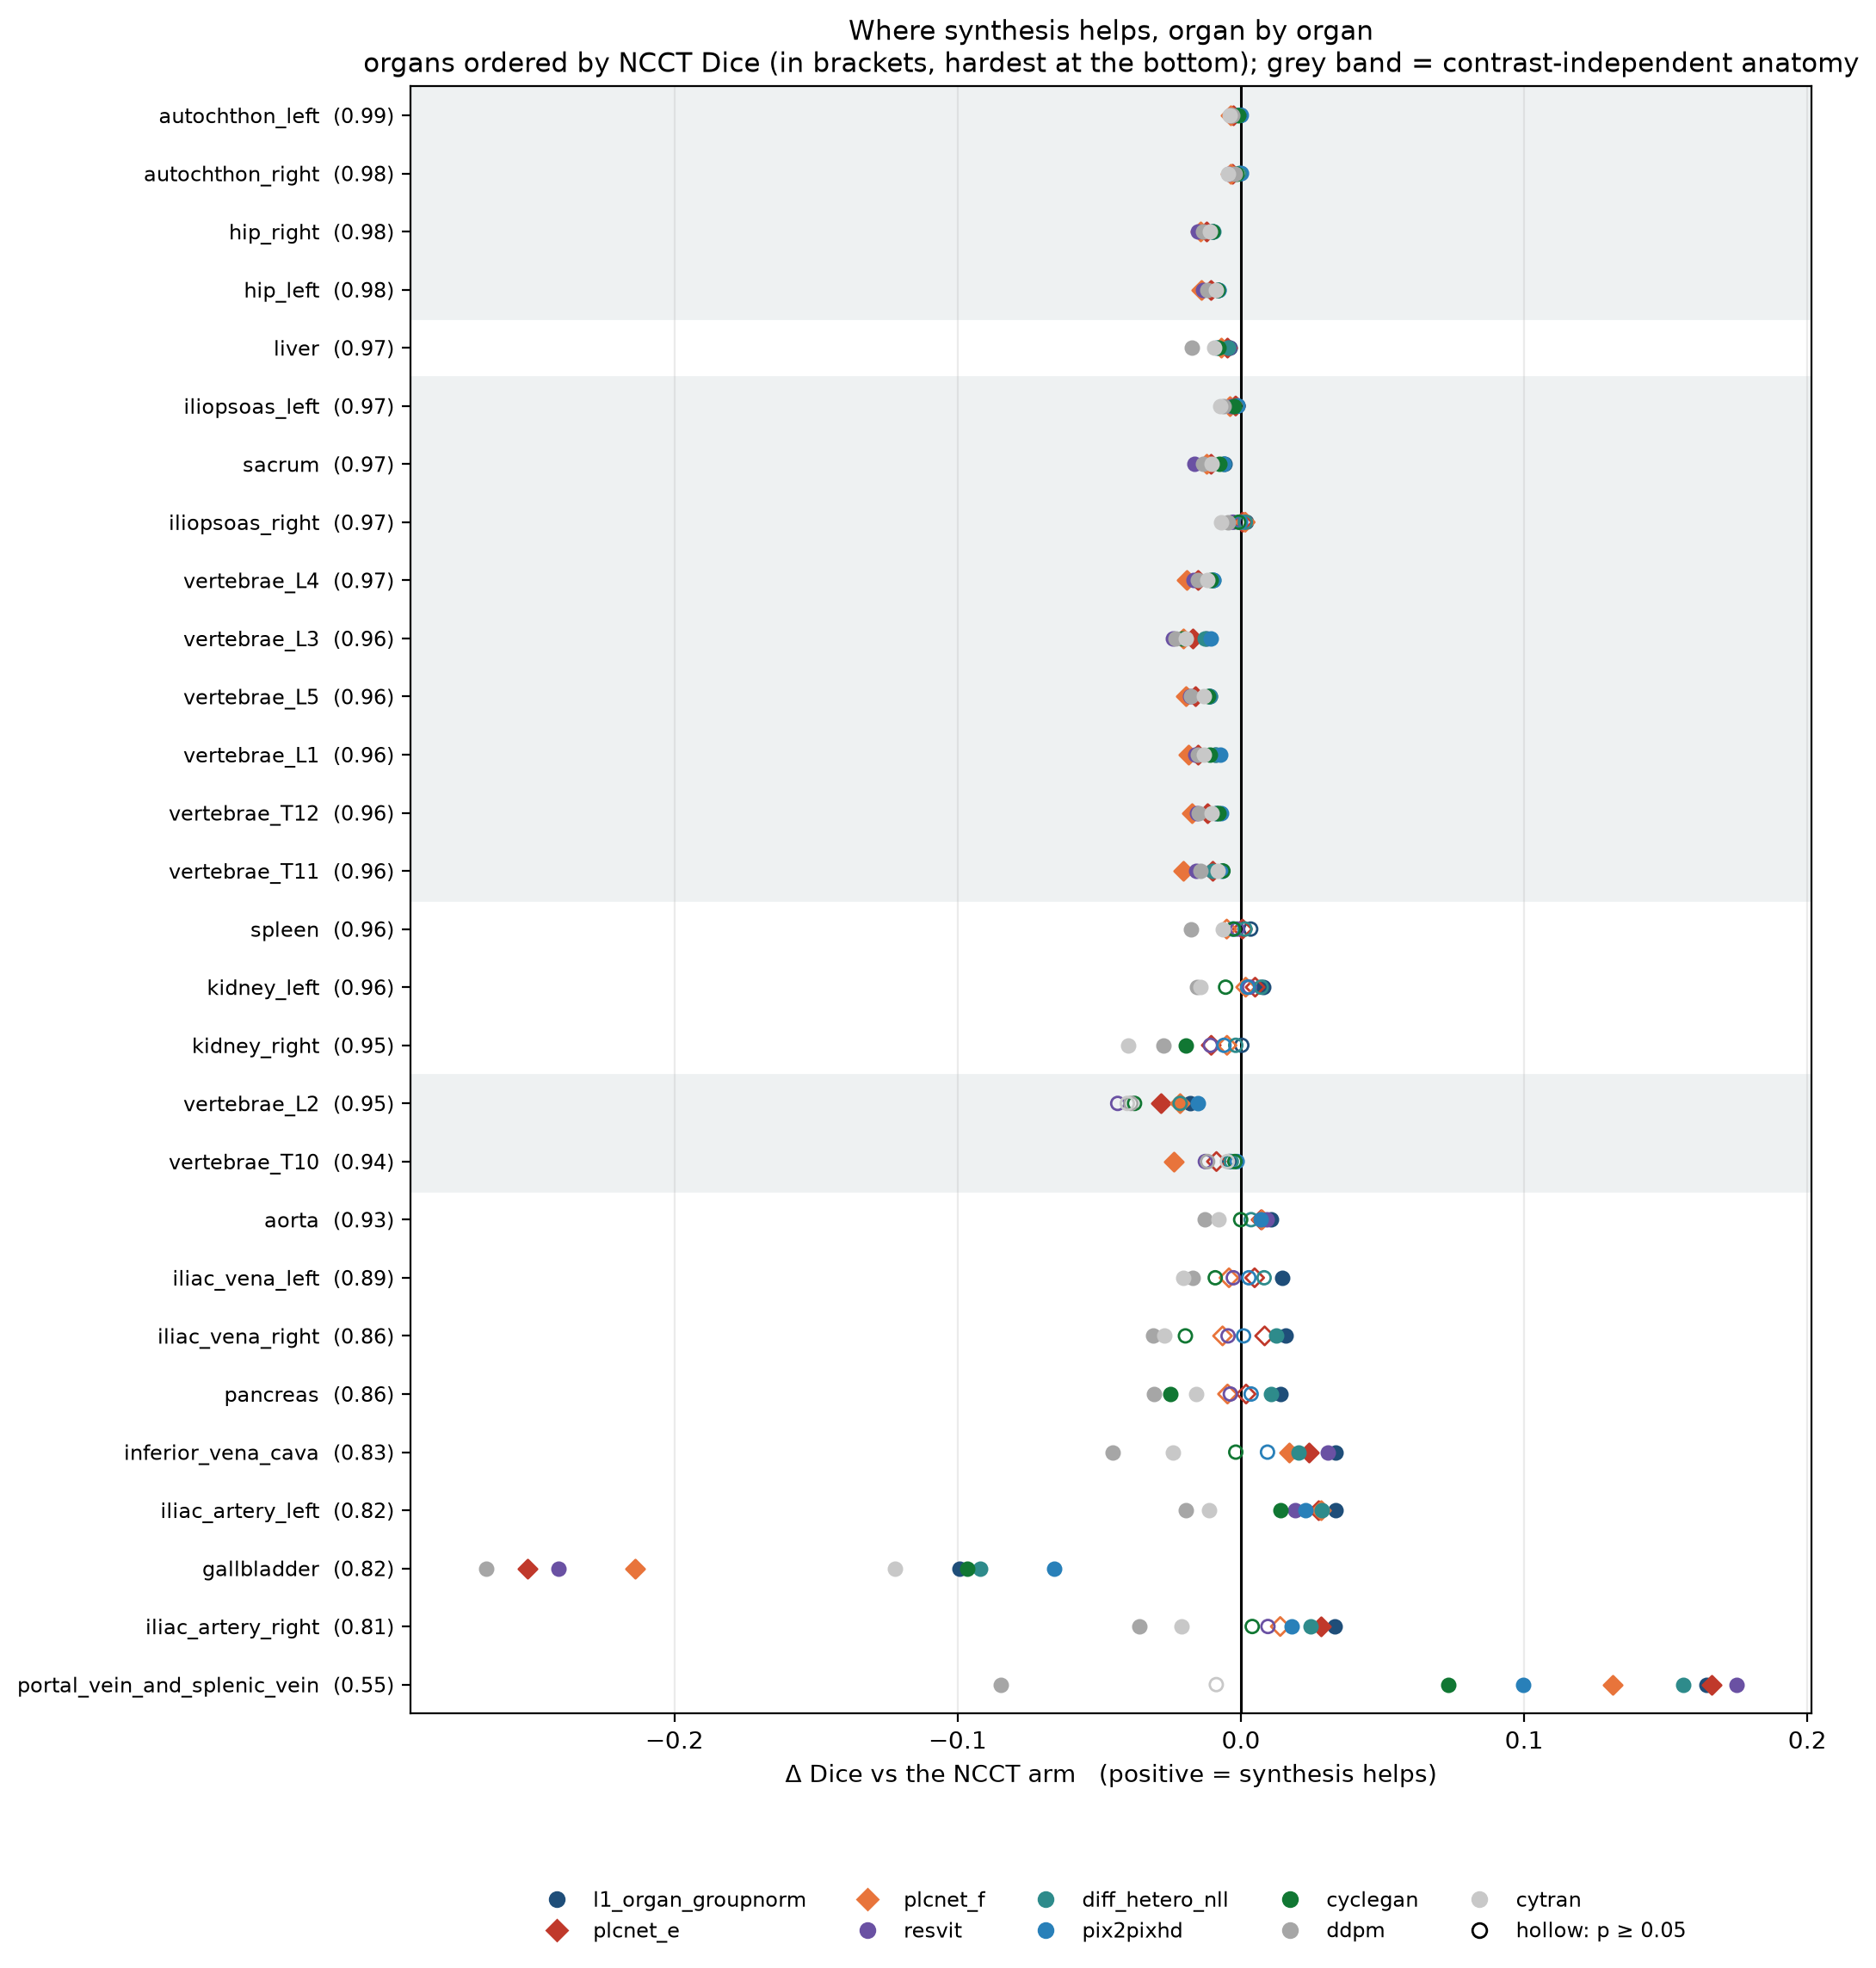
\includegraphics[width=0.82\linewidth]{fig1_per_organ_effect.png}
\end{figure}

\vspace{-6pt}
\textbf{چه چیزی را ثابت می‌کند:} اگر سنتز صرفاً «کیفیت کلی تصویر» را عوض می‌کرد، نقطه‌ها در همه‌ی سطرها به یک اندازه جابه‌جا می‌شدند. اما نوار خاکستری تقریباً روی صفر می‌ماند و کل حرکت در سطرهای پایین (عروق) جمع شده است. اثر روی ورید باب \lr{+0.13} تا \lr{+0.18} است، در ورید اجوف تحتانی و آئورت کم می‌شود، در پارانشیم به صفر می‌رسد و روی استخوان و عضله به یک کسری کوچک و یکنواخت تبدیل می‌شود. \emph{اثر متمرکز است و نه یکنواخت} \raisebox{1pt}{---} و همین شکلِ توزیع، نه بزرگی‌اش، ادعای «اثر کنتراست است و نه کیفیت تصویر» را می‌سازد.

\vspace{6pt}
\sub{۵٫۲ آیا شرط‌گذاری فاز واقعاً کار می‌کند}
هر خط یک مدل شرطی است که دو بار امتیاز گرفته: یک‌بار با شرط وریدی و یک‌بار با شرط شریانی، هر دو بار در برابر \emph{همان} مرجع وریدی. تنها چیزی که تغییر می‌کند، فاز درخواست‌شده است.

\begin{figure}[H]
\centering
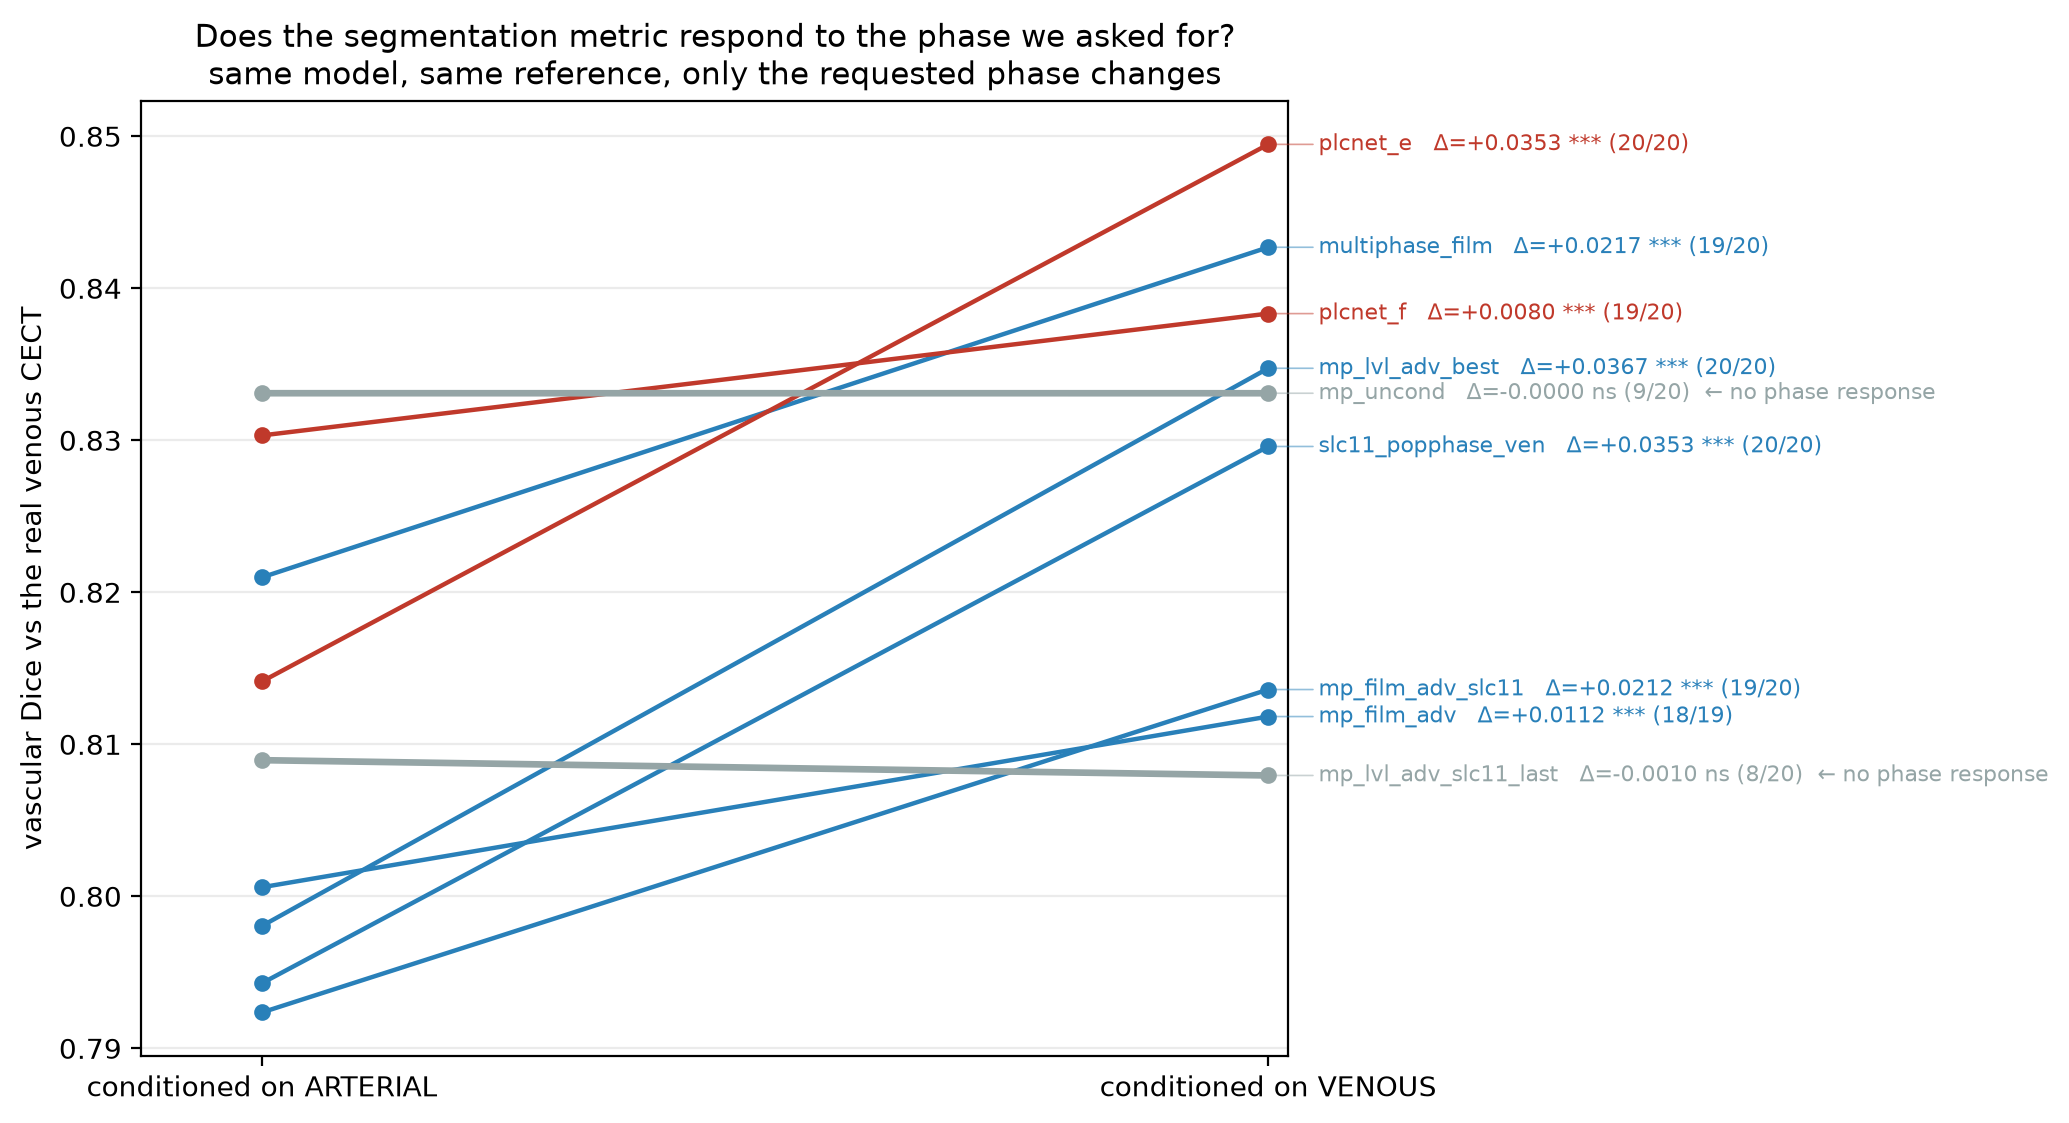
\includegraphics[width=0.92\linewidth]{fig2_phase_sensitivity.png}
\end{figure}

\vspace{-6pt}
\textbf{چه چیزی را ثابت می‌کند:} این قوی‌ترین شکل مجموعه است چون هم‌زمان سه چیز را نشان می‌دهد. (۱) هفت مدل از هشت مدل شرطی با شرط وریدی امتیاز بالاتری می‌گیرند (\lr{$\Delta$} میان \lr{+0.008} و \lr{+0.037}، همگی $p \leq 0.0002$)؛ \lr{PLC-Net} با \lr{$\Delta = +0.0353$} در ۲۰ مورد از ۲۰ مورد. (۲) \textbf{شاهد درونی:} مدل \emph{بدون شرط} ورودی فاز ندارد و نمی‌تواند درخواست را اجابت کند؛ خطش تا چهار رقم اعشار تخت است (\lr{$\Delta = -0.0000$}، $p = 0.86$). اگر آن خط شیب داشت، یعنی سنجه‌ی ما ایراد داشت. (۳) تنها اجرای شرطی‌ای که آن هم تخت است، همان اجرایی است که طبقه‌بند مستقل فاز آن را با دقت ۰٫۲۵ رد می‌کند \raisebox{1pt}{---} \emph{دو اندازه‌گیری کاملاً مستقل با هم موافق‌اند}.

\vspace{6pt}
\sub{۵٫۳ شکست شناخته‌شده: کیسه‌ی صفرا}
تنها اندامی که \emph{همه‌ی} بازوها در آن آشکارا بدتر از کف بدون‌کنتراست عمل می‌کنند. چپ: خطای علامت‌دار حجم، یک نقطه به‌ازای هر مورد. راست: دایس میانگین با نرخ تشخیص نوشته‌شده در هر ستون.

\begin{figure}[H]
\centering
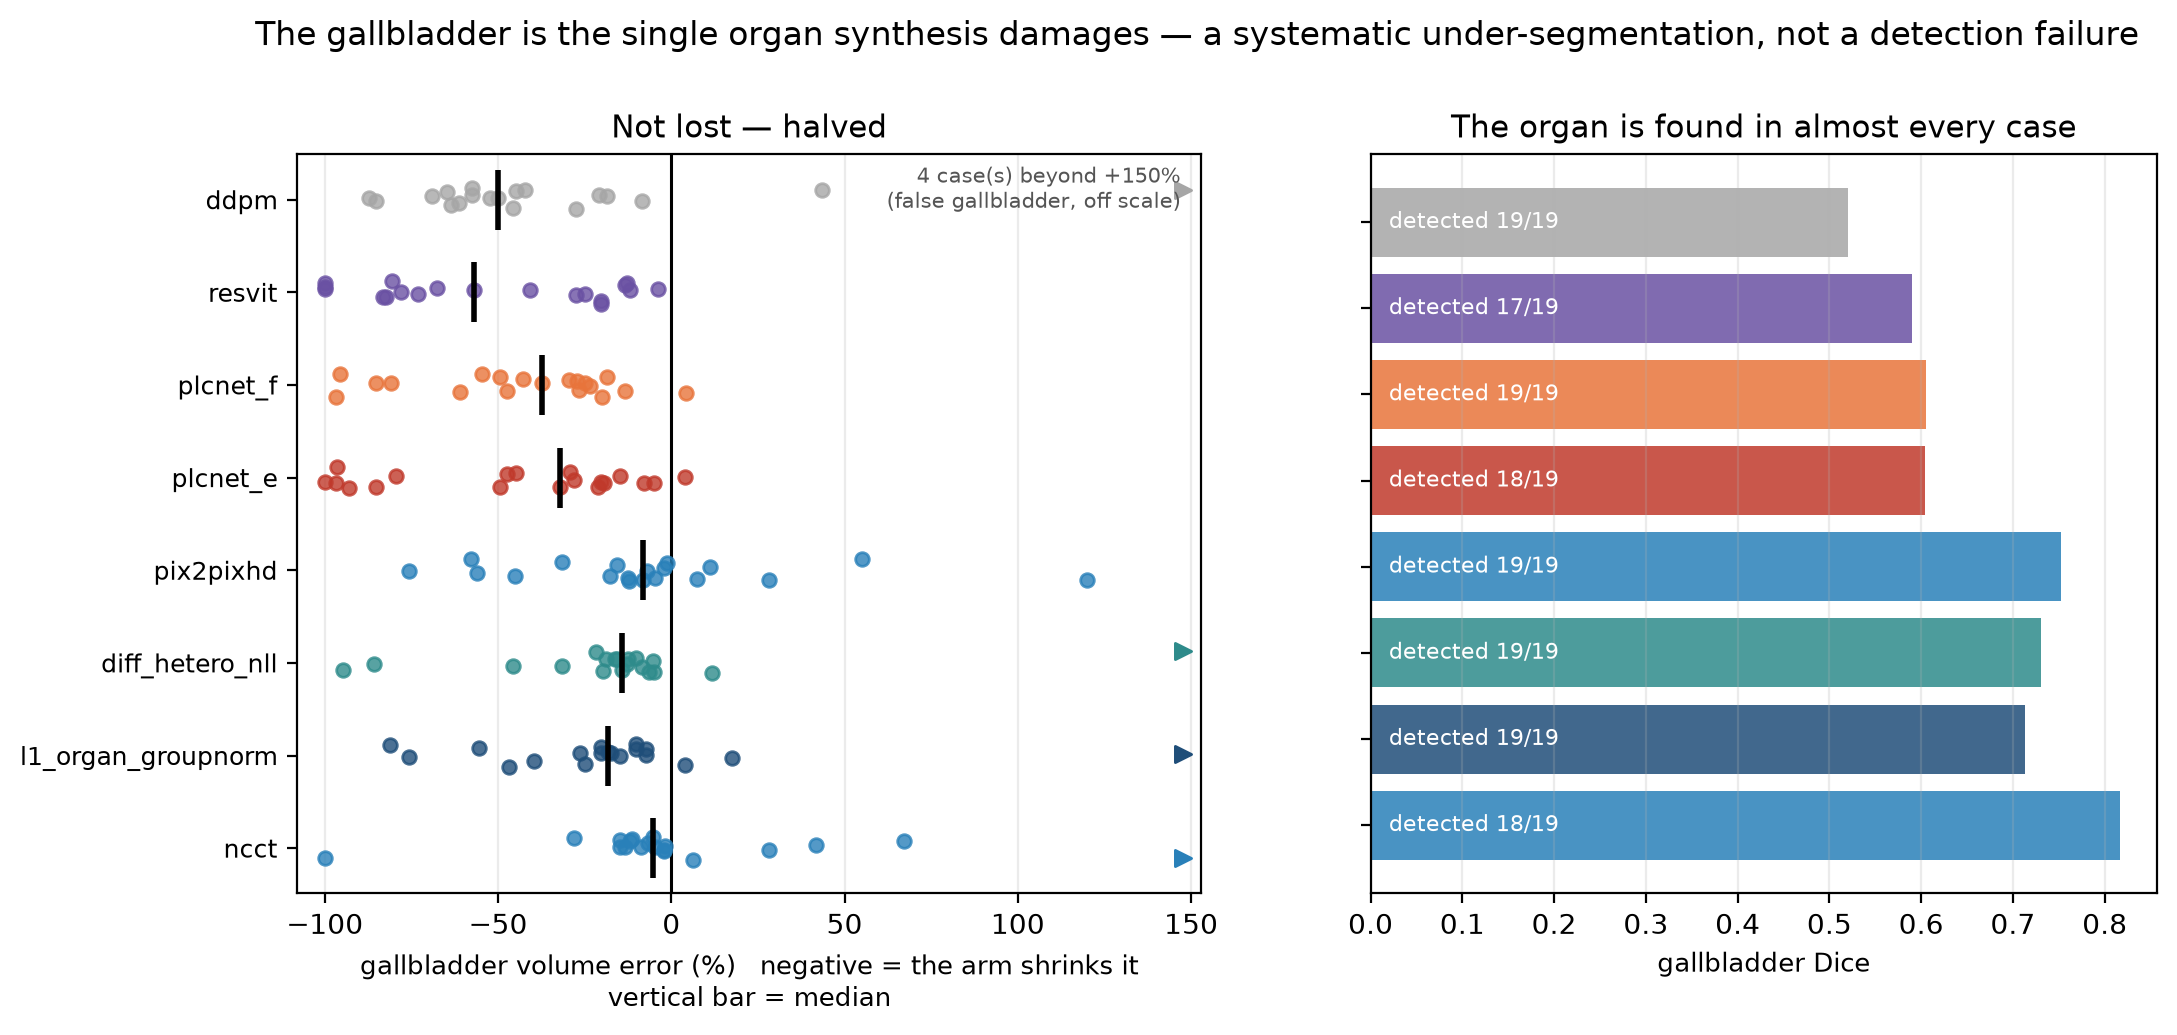
\includegraphics[width=0.92\linewidth]{fig5_gallbladder.png}
\end{figure}

\vspace{-6pt}
\textbf{چه چیزی را ثابت می‌کند:} این یک شکست \emph{تشخیص} نیست \raisebox{1pt}{---} اندام در ۱۷ تا ۱۹ مورد از ۱۹ مورد پیدا می‌شود. یک \emph{کم‌برآوردی نظام‌مند حجم} است: میانه‌ی خطای حجم از \lr{-5}٪ روی تصویر واقعی بدون‌کنتراست به \lr{-18}٪ برای \lr{l1\_organ\_groupnorm}، \lr{-32}٪ برای \lr{PLC-Net}، \lr{-37}٪ برای نسخه‌ی ۲٫۵ بعدی و \lr{-57}٪ برای \lr{ResViT} می‌رسد. تفسیر (که باید آن را تفسیر دانست و نه یافته): بازوهایی که از جمله‌ی تخاصمی و شرط سطح استفاده می‌کنند مجرای کیسه‌ی صفرا را تقویت می‌کنند، در حالی که در یک تصویر وریدی واقعی آن‌جا صفرای کم‌جذب می‌ماند و مرز از دست می‌رود. \textbf{اهمیتش:} همین یک اندام، ترکیب \lr{contrast\_critical} را از \lr{+0.166} روی ورید باب به حدود صفر در کل می‌کشاند. این را باید به‌عنوان محدودیت شناخته‌شده‌ی مدل و مشخص‌ترین جهت کار آتی گزارش کرد.

\vspace{6pt}
\sub{۵٫۴ نمونه‌ی کیفی \raisebox{1pt}{---} نوع شکست، نه اندازه‌ی آن}
ابلیشن معماری مولد روی یک برش از میانه‌ی کبد در یک مورد کنارگذاشته. هر ستون سه سطر دارد: بزرگ‌نمایی با مرز \emph{واقعی} اندام، کل برش با کادر بزرگ‌نمایی، و باقی‌مانده‌ی «تولیدشده منهای واقعی» در بازه‌ی $\pm$۱۰۰ واحد هانسفیلد (قرمز = بالاتر از واقعیت، آبی = پایین‌تر).

\begin{figure}[H]
\centering
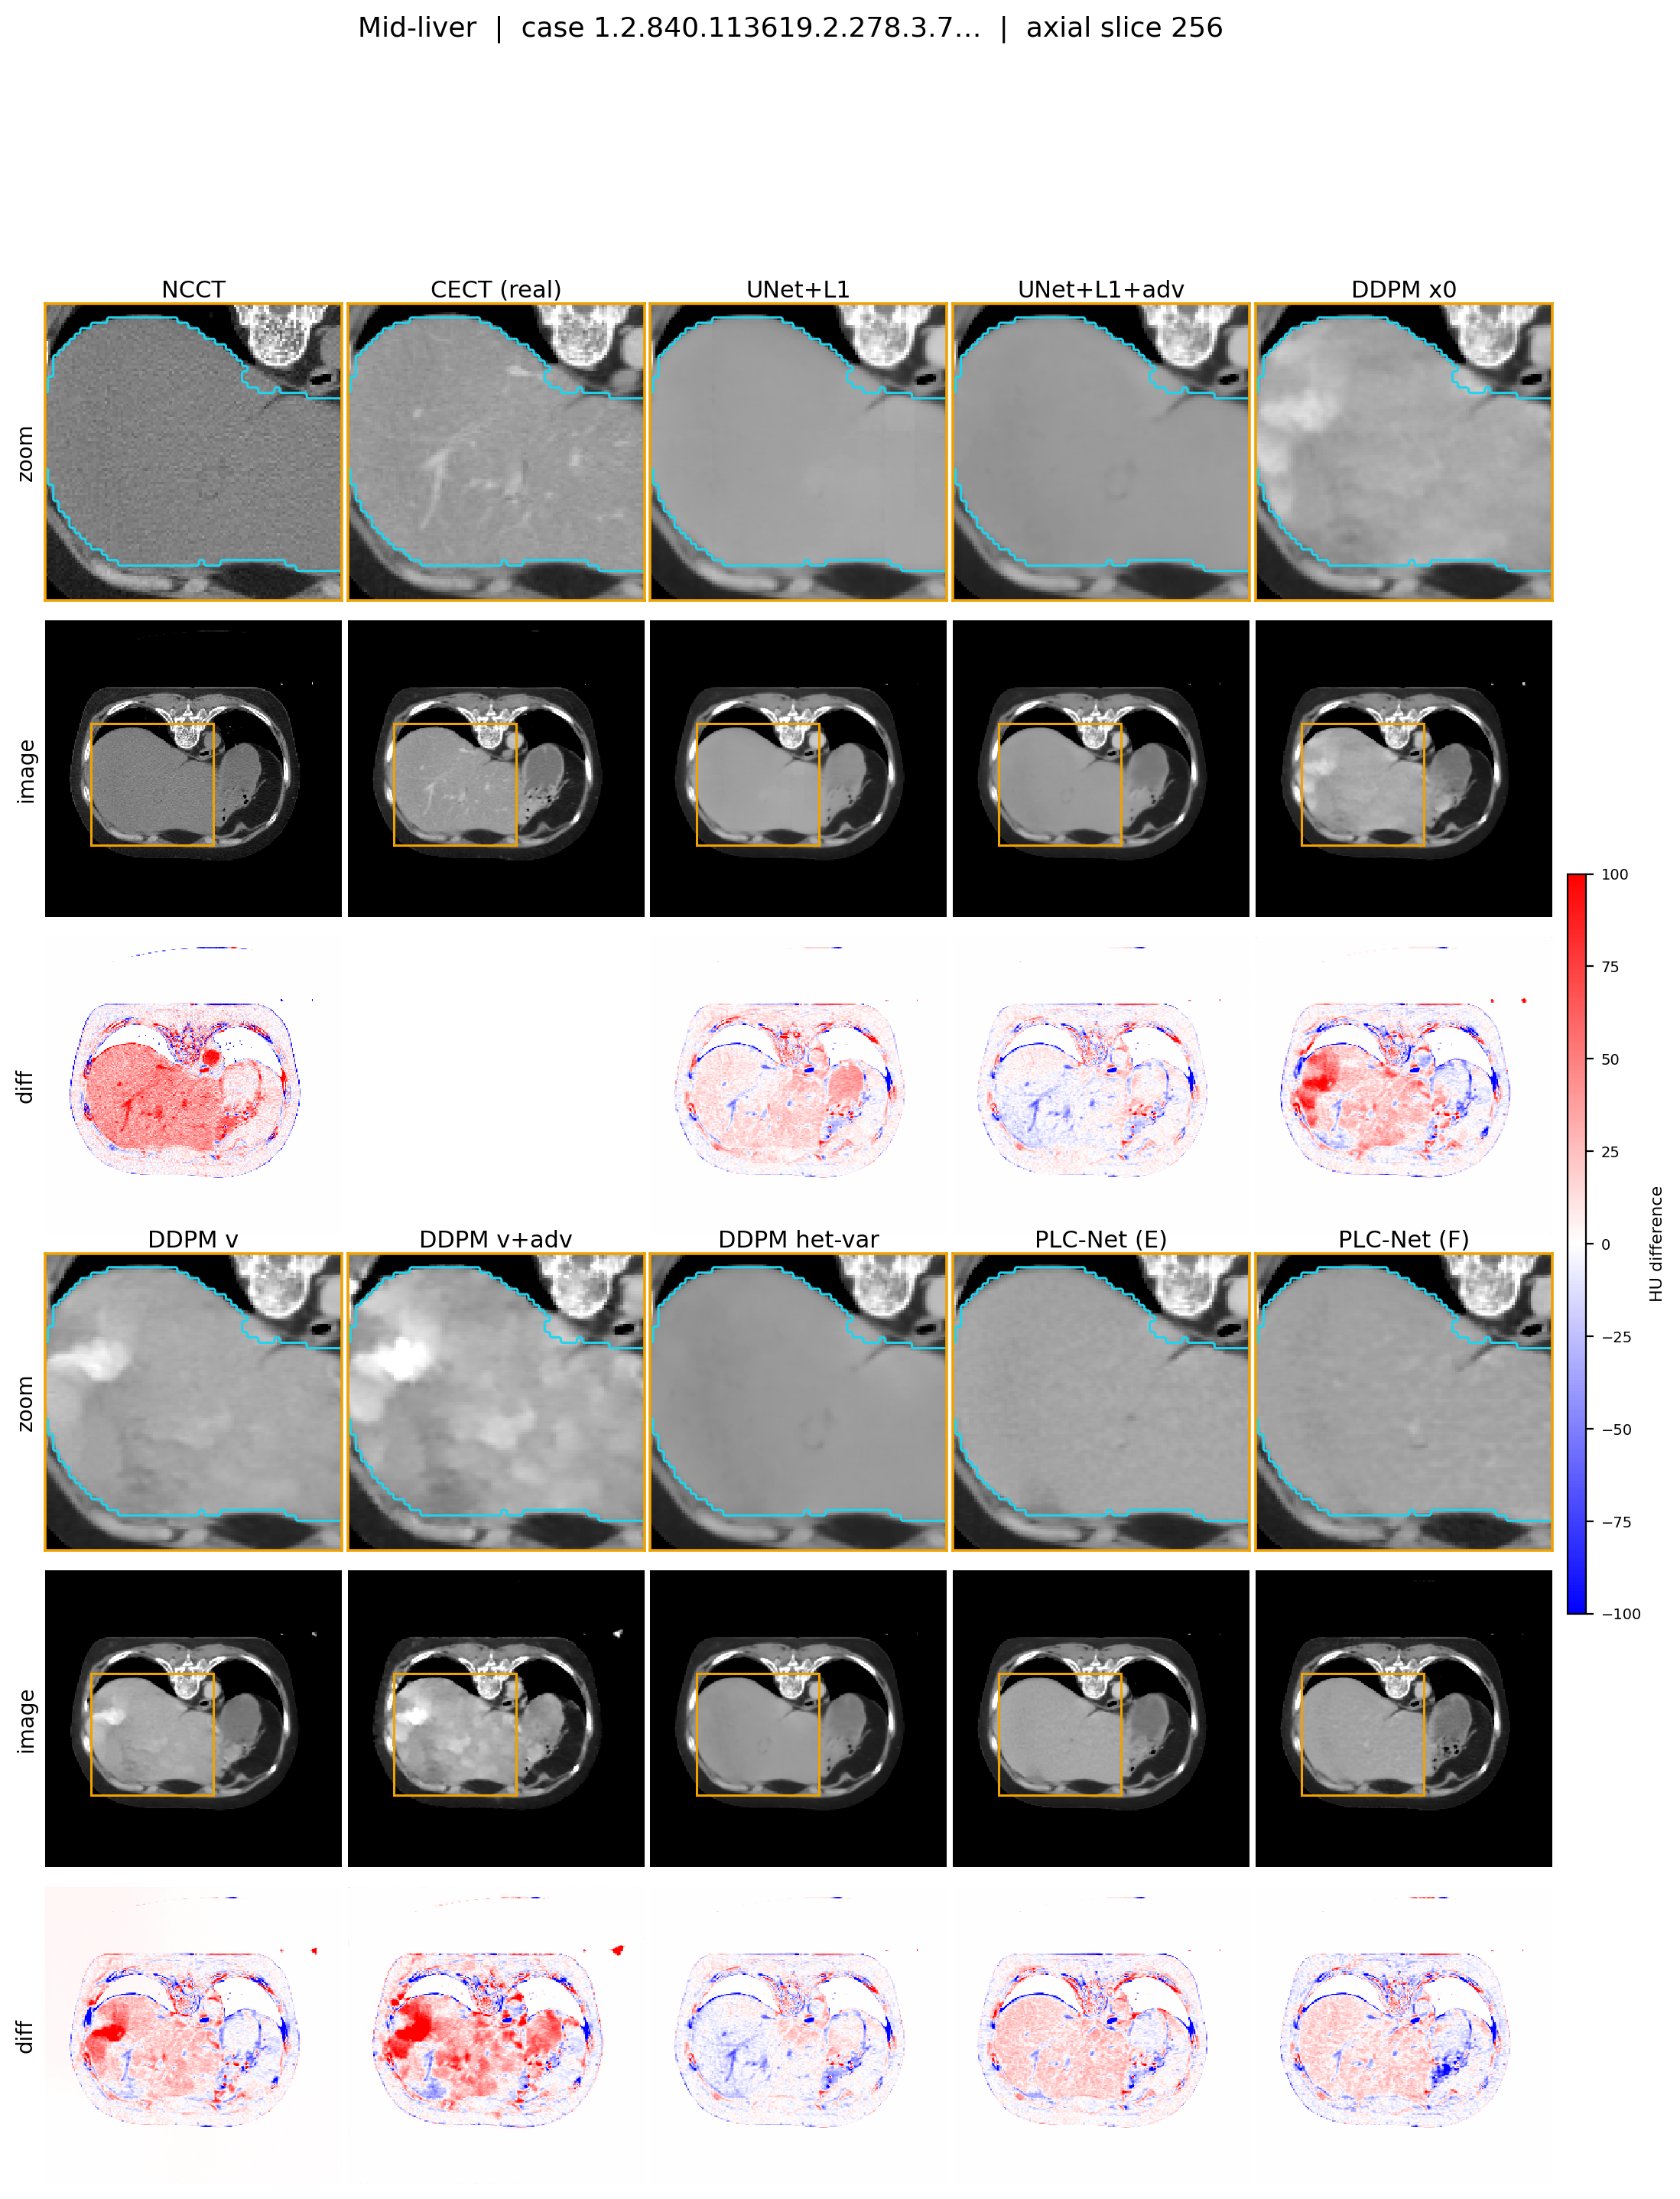
\includegraphics[width=0.88\linewidth]{ablation_mid_liver_panels.png}
\end{figure}

\vspace{-6pt}
\textbf{چه چیزی را ثابت می‌کند:} دو شکست در دو جهت مخالف، که هیچ عدد تجمیعی آن‌ها را از هم جدا نمی‌کند. هر سه بازوی انتشار (\lr{x0}، \lr{v}، \lr{v+adv}) در لوب راست کبد \textbf{توده‌ای روشن و مرزدار با ظاهر ضایعه} می‌سازند که نه در تصویر بدون‌کنتراست هست و نه در تصویر واقعی کنتراست‌دار. معیارهای پیکسلی تقریباً آن را نمی‌بینند (\lr{PSNR} برابر \lr{28.74} در برابر \lr{29.64}؛ کمتر از یک دسی‌بل)، اما \lr{featHU} می‌بیند (\lr{24.8} در برابر \lr{14.6}) و سنجه‌ی پایین‌دستی علامت را وارونه می‌کند (\lr{-0.019} در برابر \lr{+0.052}). در جهت مخالف، \lr{UNet+L1} بدون جمله‌ی تخاصمی پارانشیم را صاف می‌کند و بافت کبد و عروق درون‌کبدی محو می‌شوند. \textbf{و یک تنش صادقانه:} همین بازوی صاف، بهترین \lr{featHU} و بهترین اثر پایین‌دستی را دارد \raisebox{1pt}{---} یعنی «واقعی‌تر به نظر رسیدن» و «مفیدتر بودن» این‌جا هم از هم جدا می‌شوند. این محدودیت \emph{سنجه} است و نه برتری تاری.


\end{document}
